\chapter{Introduction}

\epigraph{La simplicité est la sophistication suprême.}{Leonardo da Vinci}

\begin{mdframed}[backgroundcolor=lightgray!30, linewidth=0pt, innertopmargin=10pt, innerbottommargin=10pt, leftmargin=10pt, rightmargin=10pt]
\small
Ce chapitre présente le contexte général du projet SecuCom, les objectifs du travail, la méthodologie adoptée et la structure du document. Il pose les bases nécessaires à la compréhension des enjeux et de la portée de ce Travail de Fin d'Études.
\end{mdframed}

\vspace{0.5cm}

À l'heure où la digitalisation des processus administratifs devient incontournable pour les entreprises, les secrétariats sociaux font face à des défis croissants en matière de gestion des données et de communication avec leurs clients. En Belgique, la complexité des réglementations sociales et la nécessité d'un traitement rapide et fiable des déclarations d'emploi (DIMONA) exigent des solutions informatiques adaptées et performantes. Pourtant, de nombreux secrétariats sociaux indépendants continuent de fonctionner avec des processus manuels, générant inefficacités, erreurs et perte de temps considérable.

\begin{figure}[h]
\centering
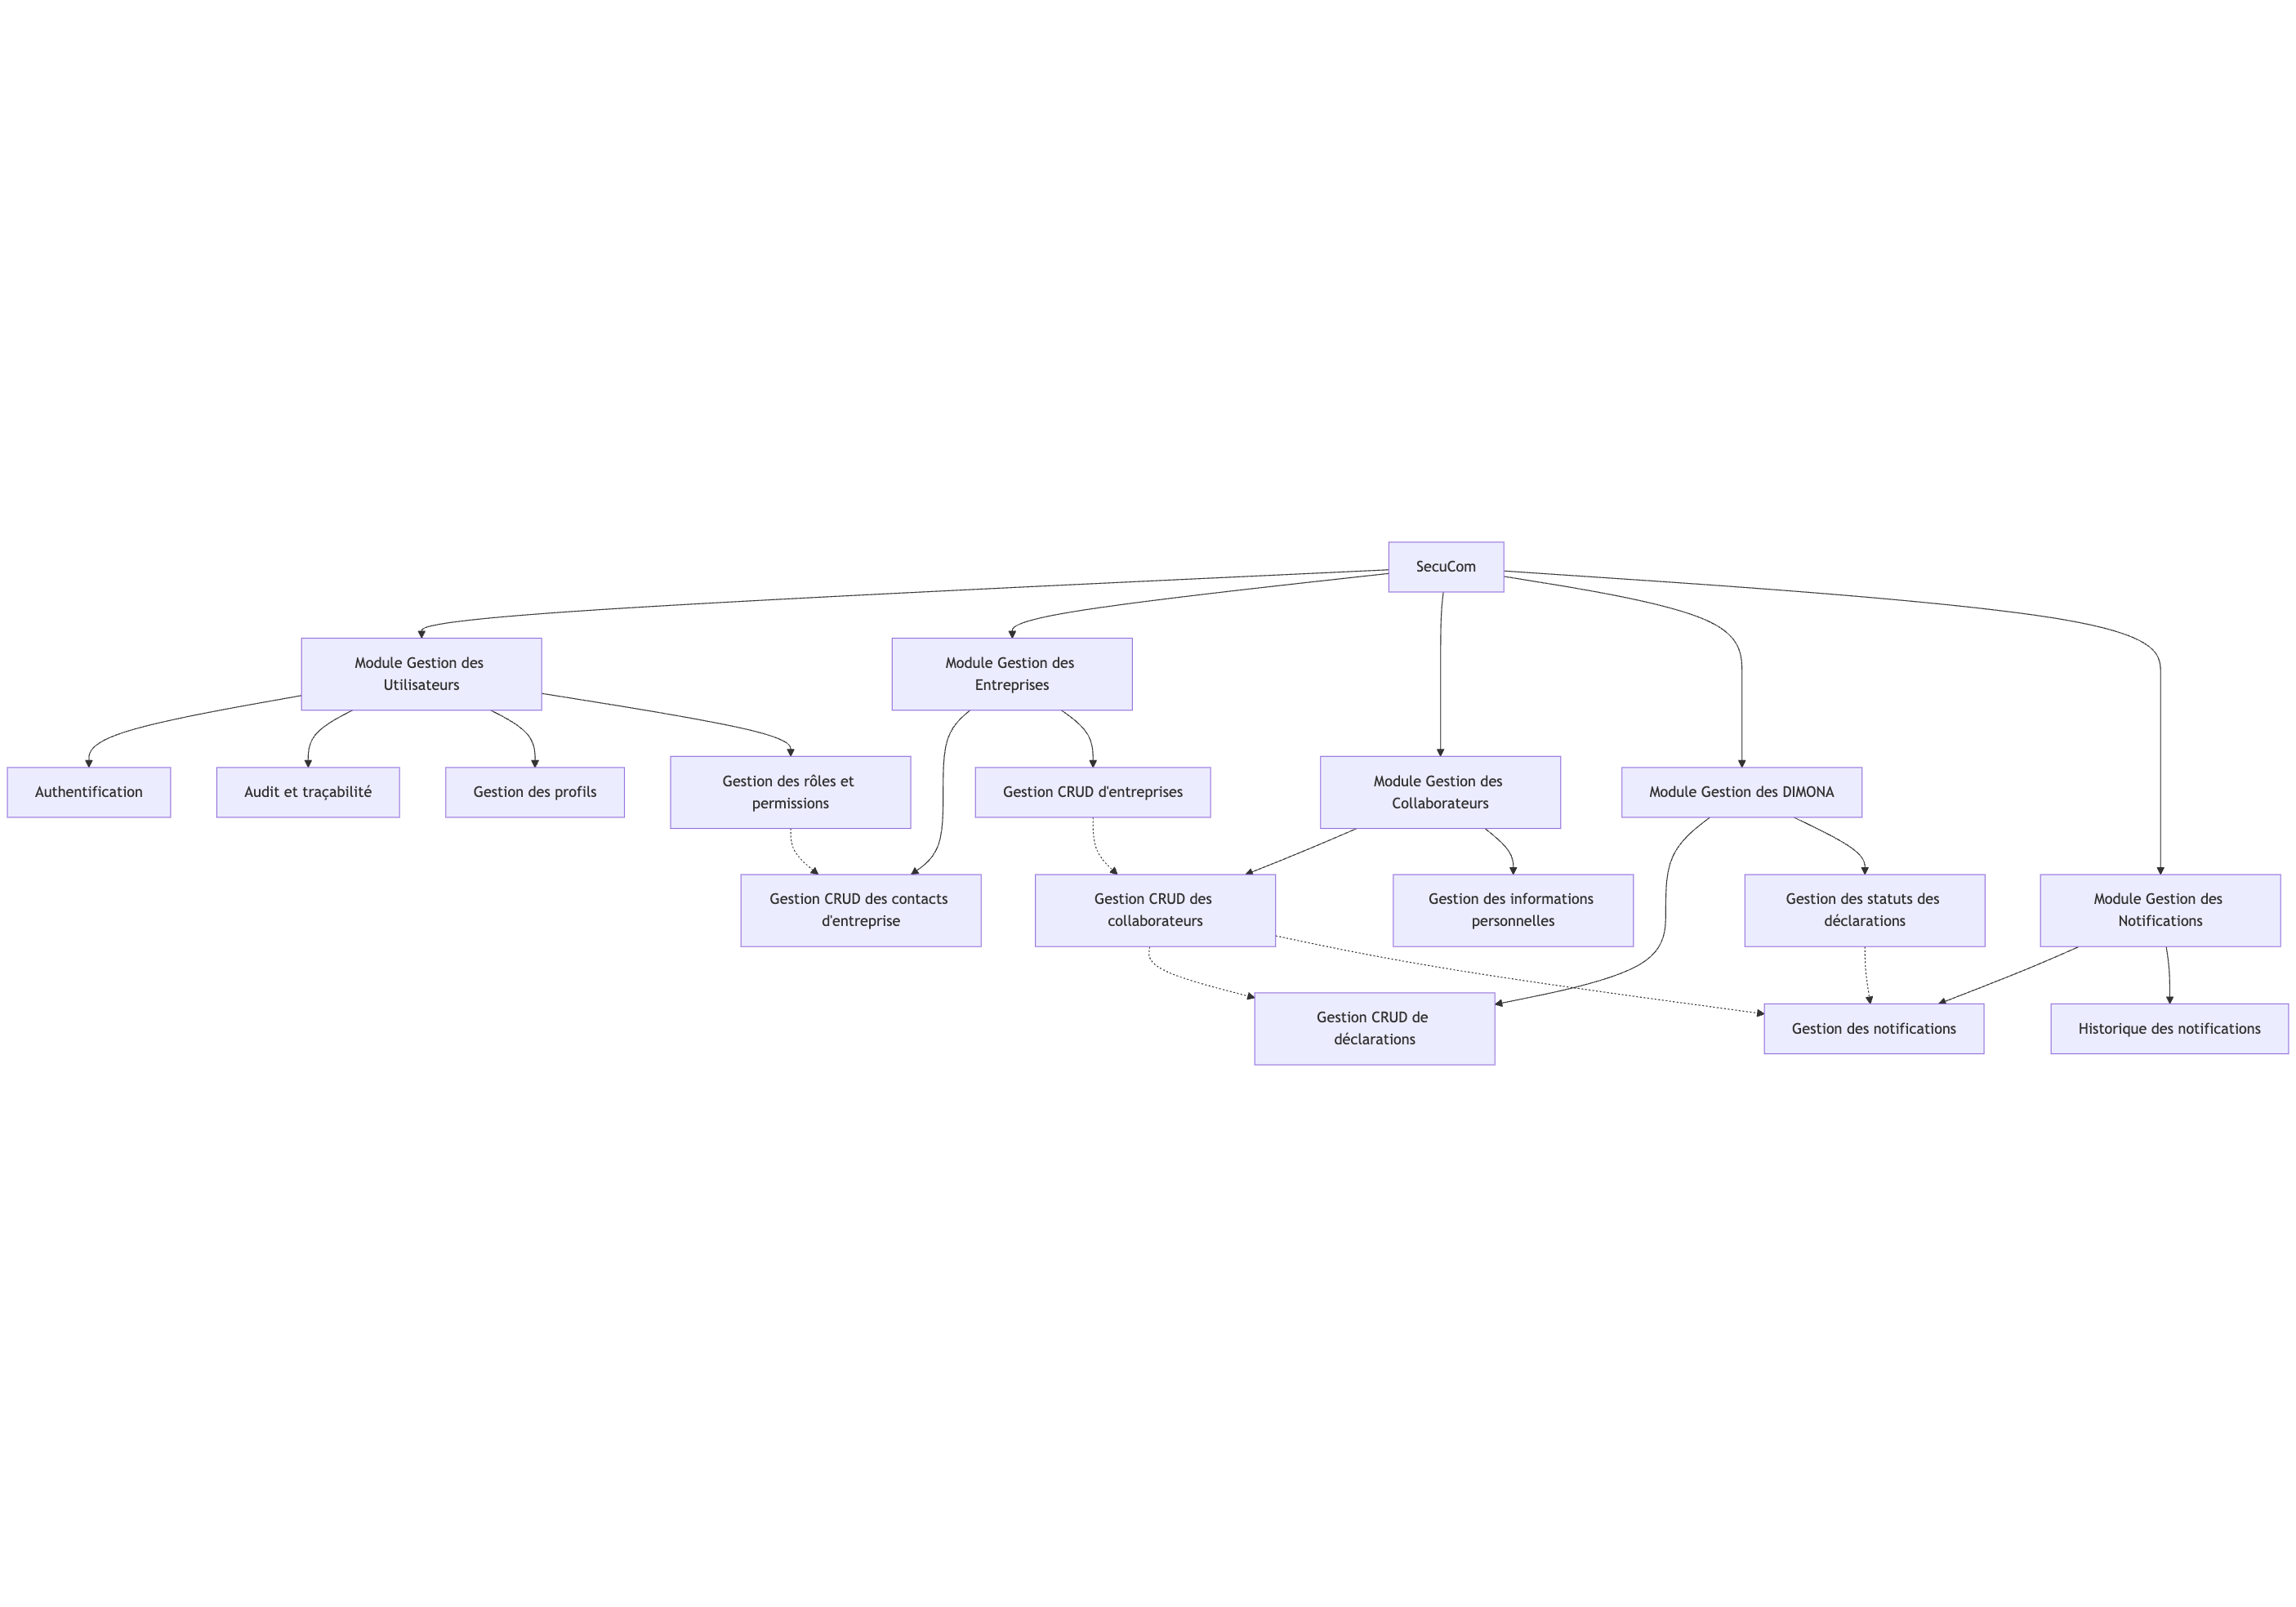
\includegraphics[width=0.7\textwidth]{ComposantsDiagram.png}
\caption{Vue d'ensemble des composants principaux de SecuCom}
\label{fig:composants-overview}
\end{figure}

\section{Objectifs du TFE}

Ce Travail de Fin d'Études, présenté à l'ISFCE dans le cadre de l'obtention du diplôme de Bachelier en informatique à orientation développement d'applications, a pour objectif de concevoir, développer et valider une plateforme de gestion pour secrétariats sociaux, baptisée \textbf{SecuCom}. Cette solution est spécifiquement adaptée aux besoins de Sodabel, un secrétariat social indépendant avec lequel une collaboration étroite a été établie.

\begin{infobox}
\textbf{SecuCom} est une plateforme web sécurisée qui vise à simplifier et optimiser les processus administratifs des secrétariats sociaux indépendants, en se concentrant sur les fonctionnalités essentielles sans la complexité des solutions existantes sur le marché.
\end{infobox}

Plus précisément, ce TFE vise à :
\begin{itemize}
  \item Analyser les processus internes de Sodabel concernant la gestion des entreprises clientes, de leurs employés et des déclarations DIMONA
  \item Concevoir une architecture backend robuste et sécurisée répondant aux besoins spécifiques identifiés
  \item Implémenter les fonctionnalités clés permettant de fluidifier les processus d'encodage et de gestion
  \item Valider la solution à travers des tests fonctionnels et de sécurité
  \item Fournir un premier jet d'une solution qui pourra être développée davantage dans un cadre professionnel futur
\end{itemize}

L'ambition de ce projet dépasse le simple cadre académique : il s'agit de proposer une solution réellement opérationnelle qui pourra être déployée et améliorée progressivement pour répondre aux besoins concrets d'un secrétariat social en activité.

\begin{definition}
\textbf{DIMONA} (Déclaration Immédiate/Onmiddellijke Aangifte) est un système belge de déclaration électronique obligatoire qui doit être effectuée par l'employeur pour tout travailleur avant le début de sa prestation de travail. Cette déclaration permet à l'ONSS (Office National de Sécurité Sociale) de connaître immédiatement quels travailleurs sont employés par quel employeur.
\end{definition}

\section{Méthodologie}

Pour atteindre ces objectifs, ce travail s'articule en quatre étapes principales, illustrées dans la Figure \ref{fig:methodologie}.

\begin{figure}[h]
\centering
\begin{tikzpicture}[node distance=2cm, auto]
% Nodes
\node[draw, fill=primarycolor!20, rounded corners, text width=3cm, align=center] (analyse) {Analyse des besoins};
\node[draw, fill=primarycolor!20, rounded corners, text width=3cm, align=center, right=of analyse] (conception) {Conception};
\node[draw, fill=primarycolor!20, rounded corners, text width=3cm, align=center, right=of conception] (implementation) {Implémentation};
\node[draw, fill=primarycolor!20, rounded corners, text width=3cm, align=center, right=of implementation] (validation) {Validation};

% Arrows
\draw[thick, ->] (analyse) -- (conception);
\draw[thick, ->] (conception) -- (implementation);
\draw[thick, ->] (implementation) -- (validation);
\draw[thick, ->] (validation) to[bend right=45] (analyse);
\end{tikzpicture}
\caption{Méthodologie de développement itérative adoptée pour le projet}
\label{fig:methodologie}
\end{figure}

\begin{itemize}
  \item \textbf{Analyse des besoins} : Plusieurs entretiens ont été menés avec les responsables de Sodabel, tant en présentiel qu'à distance, afin d'identifier précisément les points de friction dans les processus actuels. Cette phase a permis de comprendre les flux de travail existants (principalement basés sur WhatsApp et email) et leurs limitations.

  \item \textbf{Conception} : À partir des besoins identifiés, des spécifications fonctionnelles et techniques ont été élaborées, accompagnées d'une modélisation UML complète. Les choix technologiques ont été effectués en tenant compte des contraintes spécifiques du projet et des compétences disponibles.

  \item \textbf{Implémentation} : Le développement du backend a été réalisé en suivant les bonnes pratiques de développement, avec une attention particulière portée à la sécurité des données sensibles et à la séparation des espaces privés entre le secrétariat social et ses clients.

  \item \textbf{Validation} : Des tests ont été mis en place pour vérifier le bon fonctionnement des fonctionnalités développées et s'assurer que la solution répond effectivement aux problématiques identifiées lors de la phase d'analyse.
\end{itemize}

\begin{note}
Une approche itérative a été privilégiée, permettant des retours réguliers vers les phases précédentes pour affiner la solution en fonction des retours utilisateurs et des contraintes techniques découvertes en cours de développement.
\end{note}

\section{Structure du document}

Le corps de ce TFE s'articule autour de plusieurs sections qui suivent la progression logique du projet, comme illustré dans la Table \ref{tab:structure}.

\begin{table}[h]
\centering
\begin{tabular}{|p{4cm}|p{8cm}|}
\hline
\rowcolor{primarycolor!20}
\textbf{Section} & \textbf{Contenu principal} \\
\hline
\textbf{Contexte} & Environnement des secrétariats sociaux en Belgique, focus sur Sodabel et ses problématiques actuelles \\
\hline
\textbf{Description du sujet} & Présentation détaillée de SecuCom, ses objectifs et son mode de fonctionnement \\
\hline
\textbf{Analyse de l'existant} & Comparaison avec les solutions existantes (EasyPay, Liantis, etc.) \\
\hline
\textbf{Exigences et besoins} & Besoins métier, techniques et de sécurité \\
\hline
\textbf{Analyse} & Traduction des exigences en analyse UML \\
\hline
\textbf{Conception} & Choix architecturaux et design patterns \\
\hline
\textbf{Développement} & Implémentation des fonctionnalités principales \\
\hline
\textbf{Aspects financiers} & Évaluation économique du projet \\
\hline
\textbf{Conclusion} & Synthèse et perspectives d'évolution \\
\hline
\end{tabular}
\caption{Structure et contenu principal du document}
\label{tab:structure}
\end{table}

La section \textbf{Contexte} présente l'environnement des secrétariats sociaux en Belgique, avec un focus particulier sur Sodabel et ses problématiques actuelles : processus manuels chronophages, communication dispersée entre WhatsApp et emails, et risques d'erreurs élevés.

La section \textbf{Description du sujet} expose en détail SecuCom, ses objectifs et son mode de fonctionnement, en mettant l'accent sur sa simplicité d'utilisation et son interface intuitive, conçues spécifiquement pour répondre aux besoins identifiés.

L'\textbf{Analyse de l'existant} confronte notre proposition aux solutions existantes comme EasyPay ou Liantis, en soulignant comment SecuCom se distingue par son approche minimaliste et ciblée, contrairement aux solutions plus complexes et coûteuses du marché.

Les sections \textbf{Exigences et besoins} et \textbf{Analyse} présentent respectivement les besoins métier, techniques et de sécurité, puis traduisent ces exigences en une analyse précise à l'aide de diagrammes UML.

Les parties \textbf{Conception} et \textbf{Développement} abordent les choix architecturaux et décrivent l'implémentation des principales fonctionnalités : création d'entreprises, gestion des employés et traitement des déclarations DIMONA.

Enfin, les sections \textbf{Aspects financiers} et \textbf{Conclusion} proposent une évaluation économique et une synthèse qui ouvre sur les perspectives d'évolution de la solution, notamment dans le cadre d'une collaboration professionnelle future.
